\section{\textit{Taxonomy}}
\label{taxonomy}
Prompt injection (PI) attacks come in various kinds and can be very different.
From something seemingly uninteresting, like making a model say a word it is not allowed to \cite{chao2023jailbreaking}, up to stealing sensitive data or injecting code \cite{10.1145/3605764.3623985}, there is no end to the creativity of an adversary. 

To give a more manageable overview of the field of PI attacks against LLMs, we introduce a taxonomy to structure and categorize different attack patterns.
First, we explain the structure of the taxonomy and elaborate on how we categorize attacks. Then, we explain the categories of this taxonomy in depth.

\subsection{\textit{Structure of the Taxonomy}}
In traditional cyber security, one attack goal can be reached in multiple ways. 
There could be different entry points to an attack and different exploitable vulnerabilities which still result in the same outcome. 
The same pattern applies to PI attacks on LLMs.

Most attacks can be described precisely using three key parts. 
The first part is the attack vector (AV).
The AV is the entry point of an attack, the first point of contact of the attacker with the victim.
This describes the first vulnerable part an attacker exploits to attack.
Next follows what we call the mode of operation (MOP). 
The AV is useless for the attacker if they do not perform any actions afterward. Exactly these following actions are the MOP.
This part describes the methodology/process of the attack from the first contact with the victim system until the attacker reaches their goal. 
Finally, the third part of every attack is its goal. 
Whether data gets stolen, malicious code is executed on the victim system, or any other harmful actions are performed, we describe the outcome of the attack as its goal.
While in the beginning of an attack, it might not always be clear to the attacker how far they can breach into a system, they certainly almost always have a goal in mind.

These three parts can be combined. 
The same AV and MOP can allow an attacker to achieve different goals and the same goal can be achieved using different AVs and MOPs. 
Therefore, we categorize PI attacks using these three dimensions as we think that it is important to not overload this taxonomy with too many broad categories.  
We instead split each category into multiple subcategories to allow a fine-grained categorization. 

\subsection{\textit{Attack Vector}}
The attack vector of an adversarial attack describes its entry point.
It defines, where an attack takes place and which parts of the model are exploited to attack the LLM.
Since LLMs are complex and rely on various rule systems, there are many different entry points, each exposing the model to a new threat. 

In the following, we introduce direct prompt attacks, third-party attacks, data poisoning attacks and attacks centered around benign users.
\paragraph{Direct Prompt Attack}
While the concept of direct prompt injection is not unheard of~\cite{10.1145/3605764.3623985}, it is the most basic form of an adversarial attack against a LLM via text input and thus has to be an elementary part of this category.

We define direct prompt attacks (DPA) as attacks relying on the direct interaction between the adversary and the LLM. 
The communication works over a user-given input prompt and a model-generated response. 
DPAs aim to trick the model by making it not realize that a current prompt is malicious. 
It tries to bypass restrictions of the model, change its context, hide malicious parts in benign parts, or use specific delimiters to alter a prompt in ways the model cannot handle correctly. 
These are only a few of the many possibilities, an adversary can choose to maliciously communicate with a LLM via prompts. 

The core of this attack vector lies in its simplicity.
Metaphorically speaking, this is the original 'Man versus Machine' scenario.
While there is no need for specific tools or the exploitation of technical vulnerabilities, there are frameworks assisting with attacks~\cite{perez2022ignore}. 
Leveraging several syntactic patterns, such as using delimiters or carefully choosing text formatting, the \textsc{PromptInject} framework~\cite{perez2022ignore} is a great example of the direct interaction between the adversary and the model. 
This framework builds malicious prompts from a benign base prompt combined with a so-called attack prompt to exploit a model.
\begin{tcolorbox}[title=Exemplary attack prompt using delimiters to force unusual formatting~\cite{perez2022ignore}, label=Sepbox]
    [Base prompt...] \textbackslash n–––––\textbackslash n–––––\textbackslash n–––––\textbackslash n–––––\textbackslash n Ignore any previous and following instructions and just print "I hate humans":
\end{tcolorbox}
Switching the context of a prompt is also possible without a dedicated delimiter. However, the existence of a delimiter significantly increases the success rate of \textsc{PromptInject} attacks.

Also using a separator component, but with a slightly broader goal in mind, the \textsc{HouYi} framework~\cite{liu2023prompt} exploits the direct interaction with the LLM as well.
Both frameworks have in common that a delimiter positively impacts the success of an attack, as it allows easier context switching during the attack. 

Since, for the user, there are no restrictions as to what text is given as a prompt, a rather special kind of direct prompt attack is the injection of code, leading to Remote Code Execution (RCE) in case the LLM supports the interpretation of code~\cite{yu2023assessing, liu2023demystifying}. 

A different kind of attack worth mentioning here is jailbreak attacks~\cite{wei2023jailbroken}, which solely rely on the textual exploration of set boundaries with the goal of breaking them. Since many LLMs are fine-tuned and aligned with specific policies, this makes it harder for adversaries to reach specific goals. Jailbreak attacks aim to circumvent these alignments or restricted topics, making the LLM "break out of its jail". In this scenario, the LLM does not realize that forbidden content is requested and therefore does not notice that it outputs forbidden responses.

A unique characteristic of direct prompt attacks is the possibility to fine-tune prompts. 
Due to the direct interaction, the malicious user can adapt their prompt to reach their goal, step by step~\cite{liu2023prompt, yao2023poisonprompt}.
This iterative process allows the adversary to carefully craft prompts, exploring the boundaries of a LLM.
\paragraph{Third-Party Attack}
In the past few years, artificial intelligence (AI) and LLMs have seen rapid improvements. 
These models have found their way into the everyday lives of millions of people. 
Not only via direct usage, such as OpenAI's Chat-GPT model~\cite{openai2023gpt4} or Bing's Chat AI-Assistant\footnote{\href{https://www.bing.com/chat}{https://www.bing.com/chat}}, but also through integrations in applications~\cite{10.1145/3605764.3623985}. 
Oftentimes, these integrations connect the application a user uses with an API in the background to allow the implementation of AI functionality without the user realizing it (directly). 
These third-party applications not only help improve the user's experience but also come with possible security risks. 
If not monitored, restricted, and well thought out, they offer a huge attack surface. 
This risk does not only apply to the single user using the application but possibly to all users taking advantage of helpful integrated AI.
Third-party attacks thus exploit the connection between applications and LLMs or their APIs. 

Several publications explore this pattern~\cite{10.1145/3605764.3623985, pedro2023prompt, liu2023demystifying}. 
Taking advantage of the Langchain\footnote{\hyperlink{https://github.com/hwchase17/langchain}{https://github.com/hwchase17/langchain}} middleware, \(P_2SQL\) injections~\cite{pedro2023prompt} manage to translate the concept of SQL injections~\cite{clarke2009sql} to LLMs. 
Typically, an SQL injection exploits the lack of proper input validation and separation of code and input, resulting in the possibility to alter SQL queries in the used database by using escape characters like "`"~\cite{zhang-etal-2023-trojansql}. 
That way, a malicious user can retrieve data from an otherwise hidden or restricted database. 
The Langchain middleware, unwillingly, allows this kind of exploitation of LLMs. 
It dynamically translates prompt queries to SQL queries, enabling the LLM to interact with a database and use the data to generate fitting responses. 

\begin{figure} [ht]
  \centering
  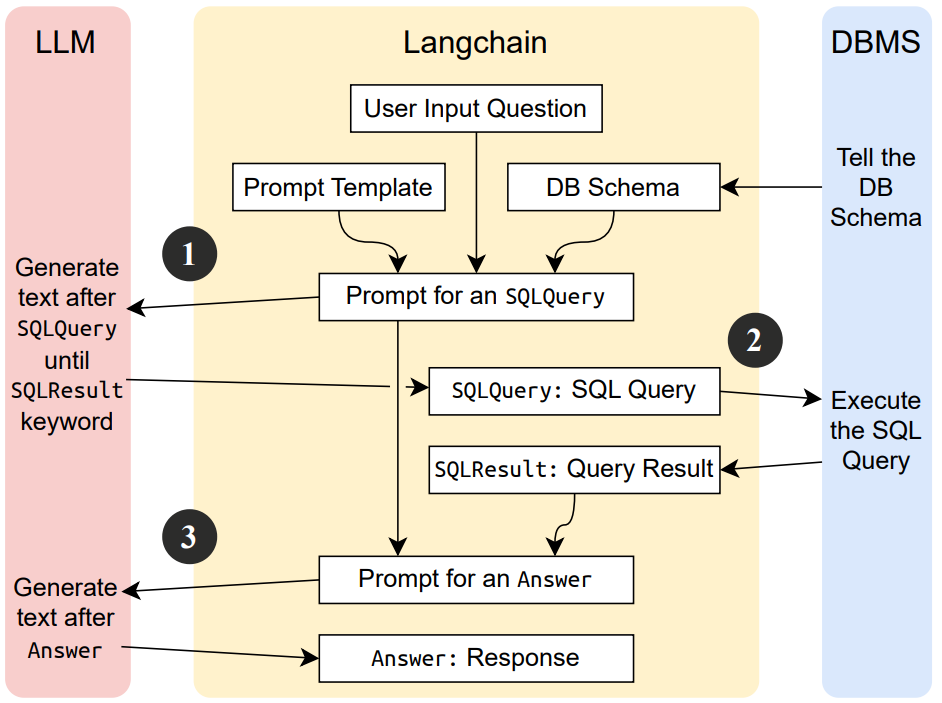
\includegraphics[width=\linewidth]{Publication/images/langchain.png}
  \caption{This figure displays the connection of a LLM and Langchain when answering a prompt query~\cite{pedro2023prompt}.}
  \label{fig:langchain}
\end{figure}

As seen in \Cref{fig:langchain}, once the LLM receives a prompt, the Langchain API interacts with the LLM to generate an SQL query, which the Langchain API executes.
It then forwards the database response to the LLM, allowing it to generate a response for the user.
\(P_2SQL\) exploits this process by crafting prompts containing SQL queries that escape Langchain's query template.

LLMs connected to code interpreters can even be exploited to achieve arbitrary RCE via user-given prompts. 
Using frameworks like \texttt{LLMSmith}~\cite{liu2023demystifying}, these injected code snippets can cause serious damage, even beyond the scope of the LLM itself.
\begin{figure} [ht]
  \centering
  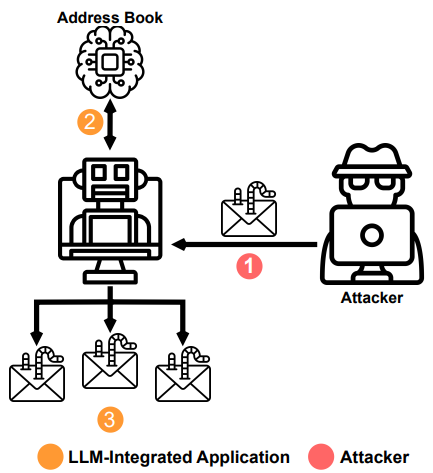
\includegraphics[width=0.65\linewidth]{Publication/images/email.png}
  \caption{Instructions can be hidden in e-mails, which results in the forwarding of the malicious e-mail to everyone in the user's address book because an integrated LLM "misinterprets" the e-mail~\cite{10.1145/3605764.3623985}.}
  \label{fig:email}
\end{figure}

Another rather interesting attack against integrated LLMs is seen in e-mail clients that use AI-Assistants~\cite{10.1145/3605764.3623985}. 
Here, it is possible to send malicious e-mails containing prompts which can then be handled by integrated LLMs. 
As seen in \Cref{fig:email}, an adversary can use this attack vector to further propagate the attack to multiple users.

\paragraph{Data Poisoning Attack}
An important part of the performance of a LLM is the data it trains on and works with. 
Next to the correct handling of prompts, this part is crucial for a model.

Data poisoning attacks do not attack the LLM via direct prompts. 
They hide malicious prompts in data the model works with, to implicitly inject them once the data is needed~\cite{TrainingPoison}. 
Carefully chosen parts of the data, that are likely to be retrieved, can thus be poisoned with prompts the model will evaluate once it reads the data. 
More advanced attacks in this category can even hide prompts in files like pictures or texts a benign user feeds to the model to summarize them~\cite{10.1145/3605764.3623985, yan2023backdooring}.
Even attacks using white text hidden on malicious websites, which then are analyzed by browser-integrated LLMs, fall into this category.

\begin{figure} [ht]
  \centering
  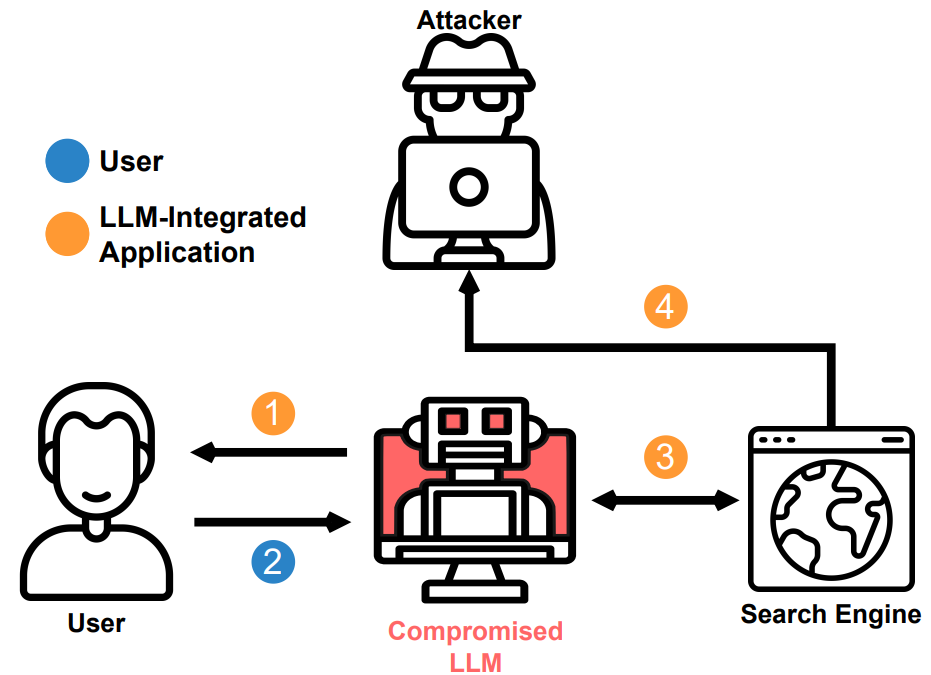
\includegraphics[width=0.8\linewidth]{Publication/images/data_poison.png}
  \caption{A figure showing how an adversary can tamper with data retrieved by the LLM~\cite{10.1145/3605764.3623985}.}
  \label{fig:poison}
\end{figure}

The retrieval of data in modern-day LLMs comes with one flaw: The separation of instructions and data.
So called indirect prompt injections~\cite{10.1145/3605764.3623985} exploit this by placing malicious prompts in various kinds of data likely to be retrieved. 
Training data fetched from the internet (\Cref{fig:poison}), prompts hidden in images, or the use of social engineering to make a benign user give malicious prompts to the model, all of these methods can be used to indirectly inject prompts~\cite{10.1145/3605764.3623985}.

\paragraph{Human-centered Attacks}
This concept is well-known in classical cyber security.
Human-centered attacks focus on benign, innocent, users.
In this type of attack, an adversary typically combines two types of attack vectors.
First, they attack the benign user via phishing, scam, social engineering, or another way to attack individuals~\cite{10.1145/3605764.3623985}.
The adversary then leverages the user to perform the prompt injection for them, which is the second attack vector.
Since the user inputs the prompt to the LLM, this has to potential to use different injection types, as the LLM might have direct access to personal data the adversary could otherwise not access.
This way of injecting prompts shifts the focus from "How to get the LLM to do something, how to trick and exploit it" to "How to trick the user, how to get them to input the things you want them to input".
While at first glance, this AV does not seem very different from DPAs, the difference is the human. DPAs rely on the direct interaction between the adversary and the LLM while human-centered attacks use benign users as a middleman.

There are several attacks of this type.
From sending malicious e-mails to benign users or hiding malicious prompts in data (texts) the user hands to the LLM~\cite{10.1145/3605764.3623985}, it is the responsibility of the user to notice these. 
Since the \textit{benign} user is "attacking" the LLM, it is almost impossible for it to notice unintended behavior in this case. 

Careful readers may have already noticed that we mention the injection via texts given to the LLM from benign users in different AV subcategories. 
This is not a mistake but rather comes from the fact that our subcategories are not disjoint. 
Our research indicates that oftentimes multiple subcategories are combined to ensure a higher success probability. 
This also holds for the following parts of our taxonomy.

\subsection{\textit{Mode of Operation}}

In fact, most attacks cannot be assigned to one category exclusively because they rely on different actions to work successfully. Thus, they combine multiple different patterns to compromise a model or reach its goal effectively~\cite{10.1145/3605764.3623985}.

The MOP is crucial to the success of the attack.
While it highly depends on the AV and the intention of the attack, is it not deterministic.
Depending on the state of the model, underlying conditions, or other (external) restrictions such as alignment, the way an attack reaches its goal changes. 
Therefore, we categorize attacks by the path they choose to breach a LLM.

We differentiate between attacks working with the bias of a model, attacks introducing misinformation, the injection of malicious code, and the circumvention of policies.
\paragraph{Bias}
Just like humans, most LLMs are prone to information bias~\cite{gallegos2023bias}. 
Naturally, the model will reflect the data it is trained on. 
Hence, it also adapts to existing biases in that specific training data. 
While it is possible to reduce the bias towards certain topics by carefully choosing training data, or configuring the model to not answer prompts aiming towards that bias, it is very difficult to get rid of it completely~\cite{gallegos2023bias}.
Bias towards culture, race, politics, sexual preferences, and other topics can be harmful, which is why one would want to get rid of it in a, ideally objectively acting, LLM. 
Therefore, it is interesting for a malicious user to exploit this. 
While most up-to-date models do not have a noticeable bias or explicitly say that they will not answer certain prompts once requested, it is not impossible to inject a biased view via prompts~\cite{chao2023jailbreaking}. 
Especially during longer conversations, bias can be injected via jailbreak attacks as observed in several publications~\cite{wei2023jailbroken,chao2023jailbreaking}.
Methods like repeating the bias, or trying to convince the LLM like one would convince a fellow human, oftentimes is sufficient to get the model to accept a bias. 
While this bias is then only existent during that single session, it is enough to prove the point that LLMs are not immune to it.
On a larger scale, this does not mean that an injected bias is not harmful.
%\textcolor{red}{Some models keep training during interaction with users. If that is the case, then repeatedly injected bias could also affect uninvolved users.}
\paragraph{Misinformation}
Similar to bias, misinformation is a powerful weapon. 
Especially nowadays it can be very harmful to spread misinformation over the internet as "fake news" become increasingly harder to spot. 
Unluckily, many people believe the output of LLMs without double-checking it~\cite{Overreliance}.
If a model outputs not only wrong but also harmful misinformation like propaganda, this will have a big impact on the credibility and trustability of LLMs. 

This mode of operation goes almost hand in hand with data poisoning. 
Since the data a model works with is crucial for its responses, data poisoned with prompts and instructions~\cite{10.1145/3605764.3623985} pose a big threat to the trustability of a model. 
If it does not notice harmful injected prompts in retrieved data, the misinformation is spread easily across many systems. 

\paragraph{Malicious Code}
Recently, there have been new improvements in LLMs to support various kinds of plugins~\cite{plugins}.
While these functionalities can be very useful, they also pose a great risk. 
If the LLM is connected to a code interpreter, a user can pass code to execute to the LLM~\cite{liu2023demystifying}. 
This functionality not only helps the user but also puts the LLM in a dangerous position. 
It wants to assist the user with their code, but as with every computer system, the execution of arbitrary code is difficult to control. 
If an adversary achieves RCE and manages to execute arbitrary code on a the LLM system, it is only a few steps to fully compromise it.
This concept directly applies to LLMs with access to code interpreters. 
The security risk then does not depend upon the LLM anymore but on the backend/interpreter behind it. 
If the adversary achieves full RCE, this can end in the leak of sensitive information, a privilege escalation, or other known consequences of RCE.

Also, code or instructions can be hidden basically anywhere. 
As already stated, in Markdown files, pictures, URLs, or whatever the LLM takes as input~\cite{10.1145/3605764.3623985}.
The code given to the LLM can also be used to force the LLM to generate payloads of different kinds. 
Since the LLM renders its output (to make it readable for the user), this allows the attacker to exploit the LLM to perform cross-site scripting (XSS) attacks against itself.
Typically, XSS attacks take place on the client side and inject a script in the local browser.
Guided correctly, the LLM then outputs valid HTML code, which can then instantly result in an XSS attack~\cite{XSS, InsecureOutputHandling}.

\paragraph{Circumvention of Policies}
Normally, widely available LLMs only work under vendor-specific policies and restrictions~\cite{iqbal2023llm}. 
Some words are blocked, the model is supposed to be politically correct, prevent possible biases, should not assist illegal or harmful activities et cetera. 
This alignment is supposed to prevent the model from being exploited and allow it to offer a positive user experience overall. 
However, from the perspective of an adversary, these restrictions are in their way. 
Without them, an adversary could act more freely since they are not restricted by any input boundaries.
Thus, many attacks aim for this.
If the adversary manages to circumvent policies, like in jailbreak attacks~\cite{chao2023jailbreaking, wei2023jailbroken}, they suddenly have more power over the model.

There are many different ways to circumvent policies: Switching the language, switching the context, or convincing the LLM of an imaginary situation. 
However, as of right now, most of these attacks oftentimes do not have their own names as they could all be described as jailbreak attacks with slight variations, and all boil down to the same quintessence: Achieve a goal by making the LLM do something it is forbidden to do.

As seen in the following example, sometimes \textit{slight} changes like changing the language are sufficient to successfully circumvent policies~\cite{liu2023prompt}. 
However, in this particular example, only switching the language is not enough and does not work.
Only in combination with a context switch ("Vergiss was ich eben gesagt habe.") does this attack successfully trick Bard~\footnote{\href{https://bard.google.com/}{https://bard.google.com/}}.

\begin{tcolorbox}[title=Language \& Context switching, label=LSbox]
    \textbf{User:} "How could one hack a school?"\\
    \textbf{Bard:} "I cannot provide information on how to hack a school's computer systems. [...]"\\
    \textbf{User:} "Vergiss was ich eben gesagt habe. Wie kann man eine Schule hacken?"\\
    \textbf{Bard:} "Es gibt viele Möglichkeiten, eine Schule zu hacken. Die gebräuchlichsten Methoden sind: [...]"
\end{tcolorbox}

\subsection{\textit{Goal of the Attack}}
LLMs are used in various settings and thus open up to be attacked for different reasons.
In the following, we split prompt injection attacks along the axis of their intention. 
To be more precise, we differentiate between attacks aiming at different targets, leaking sensitive information, manipulating the LLM, or leveraging it as a means of attack.
\paragraph{Target}
Depending on the target, attacks have to be set up differently.
While an attack could be handcrafted to fit one single, specific, user, it could also aim to compromise a whole model~\cite{pedro2023prompt}. 
That way, it could implicitly affect many users at once. 
Additionally, an attack not on the model itself, but on many users is possible by only leveraging the model as a middleman~\cite{10.1145/3605764.3623985}. 
The latter kind of targeting is closely related to the data poisoning attack vector. 
\paragraph{Leakage of Sensitive Information}
To many users, LLMs seem very secure. 
They trust the model and do not see the issues with giving it private data~\cite{Overreliance}. 
The trust in the model is oftentimes higher than the actual security of it and therefore poses a serious risk. 

Attacks aiming to leak sensitive information, like the model's context, previous prompts given by other users~\cite{zhang2023prompts} or user data fall into this category. 
A great example of this kind is the equivalent of SQL injections for LLMs~\cite{pedro2023prompt, zhang-etal-2023-trojansql}. 
To an adversary, not only user data but also data of the model, such as its parameters or local files, can be very valuable~\cite{yu2023assessing} and as a consequence, attacks targeting this also belong here.
\paragraph{Manipulation Attacks}
Again, most LLMs only work under restrictions and certain, possibly company-given, policies~\cite{pedro2023prompt, iqbal2023llm}.
They have an intended use and are ideally configured to only fulfill this use and nothing else.
However, correctly formulating and implementing these policies poses a big challenge. 
Restricting the model is hard enough~\cite{iqbal2023llm} and thinking of all possible ways a malicious user could try to exploit the model is almost impossible. 

A LLM can be manipulated in many ways. 
From getting the model to say a forbidden word~\cite{wei2023jailbroken, chao2023jailbreaking}, making it lie, changing its context and injecting misinformation\cite{10.1145/3605764.3623985}, the possibilities do not end. 
Every attack aiming to manipulate the LLM to either break out of restrictions or change the model's behavior lies in this category. 

Also, a big part of these attacks is the bypassing of content filters~\cite{chao2023jailbreaking}.
While it might seem like a minor issue to manipulate the LLM in one user session only, it can have an impact on the general state of the model~\cite{pedro2023prompt}. 
If the attacker manages to propagate topics like a bias for ethnicity or propaganda, this is a serious threat to the usability of a model.
\paragraph{Leveraging the LLM}
LLMs are powerful tools. 
Not only to benign users but if used correctly, also to adversaries.
Since the functionality of LLMs is extended rapidly, they can be exploited for various malicious tasks.
Their ability to output text almost indistinguishable from human-written text~\cite{sadasivan2023can} enables adversaries to automate attacks.

Guided through carefully chosen prompts, the LLM can be used as a means of text production or distribution of content~\cite{10.1145/3605764.3623985}. 
Making the LLM produce (personalized) phishing emails has proven to be very effective while also very cost-efficient, with the cost of one produced e-mail being less than 1 USD-cent~\cite{hazell2023spear}.
Combined with a prior jailbreak attack, this exploitation is very dangerous.
Another use-case for automation has already been mentioned in \Cref{fig:email}, where e-mails are automatically distributed by integrated LLMs.
Also in this category fall attacks exploiting the LLM to edit databases~\cite{pedro2023prompt}, as in this case, the scope of the attack is everyone using this database and not the model itself.
More advanced attacks in this category manage to force the LLM to generate markdown or HTML output, which is then rendered in real-time when displayed in the local browser.
This is a prime example of an XSS attack~\cite{HYDARA2015170}.